\documentclass[english,11pt]{beamer}

\DeclareMathOperator{\Cov}{Cov}
\DeclareMathOperator{\Var}{Var}
\DeclareMathOperator{\E}{\mathbb{E}}
\DeclareMathOperator{\Proba}{\mathbb{P}}

\newcommand{\Covb}[2]{\ensuremath{\Cov\!\left[#1,#2\right]}}
\newcommand{\Eb}[1]{\ensuremath{\E\!\left[#1\right]}}
\newcommand{\Pb}[1]{\ensuremath{\Proba\!\left[#1\right]}}
\newcommand{\Varb}[1]{\ensuremath{\Var\!\left[#1\right]}}

% norm
\newcommand{\norm}[1]{\| #1 \|}

\newcommand{\indep}{\rotatebox[origin=c]{90}{$\models$}}





\usepackage{mathptmx,amsmath,amssymb,graphicx,bibentry,bbm,babel,ragged2e}

\makeatletter

\newcommand{\noun}[1]{\textsc{#1}}
\newcommand{\jitem}[1]{\item \begin{justify} #1 \end{justify} \vfill{}}
\newcommand{\sframe}[2]{\frame{\frametitle{#1} #2}}

\newenvironment{centercolumns}{\begin{columns}[c]}{\end{columns}}
%\newenvironment{jitem}{\begin{justify}\begin{itemize}}{\end{itemize}\end{justify}}

\usetheme{Warsaw}
\setbeamertemplate{footline}[text line]{}
\setbeamertemplate{headline}{}
\setbeamercolor{structure}{fg=purple!50!blue, bg=purple!50!blue}

\setbeamersize{text margin left=15pt,text margin right=15pt}

\setbeamercovered{transparent}


\@ifundefined{showcaptionsetup}{}{%
 \PassOptionsToPackage{caption=false}{subfig}}
\usepackage{subfig}

\usepackage[utf8]{inputenc}
\usepackage[T1]{fontenc}

\usepackage{multirow}

\usepackage{mdframed}


\makeatother

\begin{document}



\title{A scientometric analysis of linkages between urban digital twins and urban simulation models}

\author{J.~Raimbault$^{1,2,3,4}$\\
\texttt{juste.raimbault@ign.fr}
}


\institute{$^{1}$LASTIG, Univ. Gustave Eiffel, IGN-ENSG\\
$^{2}$CASA, UCL\\
$^{3}$UPS CNRS 3611 ISC-PIF\\
$^{4}$UMR CNRS 8504 G{\'e}ographie-cit{\'e}s
}


\date{\textit{Journ{\'e}e de la Recherche UGE-IGN-ENSG 2024}\\
28/03/2023
}


%Following the trend of smart cities, urban systems have been under an extensive focus for the development of urban digital twins, which are particularly relevant given their complex nature, the abundance of real-time data within cities, and the difficulty of decision-making to manage and design cities over several time scales. In that context, urban simulation models, which have been largely studied for several decades, should be at the core of such approaches, following the standard definition of a twin which mirrors the processes of the twinned system, and for these to have any interest for decision-making. We propose in this contribution a scientometric analysis of effective linkages between these two streams of literature, namely urban digital twins and urban simulation models. We construct a large citation network using open bibliographic data collection tools, and find that despite the fact that many twins use simulation, connections between the fields remain relatively low. This may reflect the fact that existing twins operate mainly at a short time scale, whereas urban simulation deals with slower dynamics. This highlights the need for a higher interoperability and integration between these approaches.

% A priori bib simu
%Autres aspects simu
%Bib sys rev dig twins domaines
%Enjeu planning vs management
%Rappel last y
%Q rech liens


%Resultats :
%Grde commus
%pct par origine [cbien both]
%Composition comus par original
%Echange cits entre comes
%[Check alife paper]

%Perspective : analyse a la Florent timescales et types de modeles

%Rappel simu essentielle pour le jumeau - def 
%Positionmt oml - validation

\frame{\maketitle}


\sframe{Urban digital twins}{

% Bib sys rev dig twins domaines

}

\sframe{Urban simulation models}{

% A priori bib simu
%Autres aspects simu


}

\sframe{Research question}{

%Enjeu planning vs management
%Rappel last y
%Q rech liens

}

\sframe{Data and methods}{

% corpus construction and scim tools - cit nw

}


%Resultats :

\sframe{Citation network}{

}

\sframe{Main fields}{

%Grde commus

}

\sframe{}{

%pct par origine [cbien both]

}

\sframe{}{

%Composition comus par original

}


\sframe{}{

%Echange cits entre comes
%[Check alife paper]

}



\sframe{Perspectives}{

%Perspective : analyse a la Florent timescales et types de modeles
%Rappel simu essentielle pour le jumeau - def 
%Positionmt oml - validation


\justify

$\rightarrow$ 

\medskip

$\rightarrow$ 


}



%%%%%%%%%%%%%%%%%%%%%
\begin{frame}[allowframebreaks]
\frametitle{References}
\bibliographystyle{apalike}
\bibliography{biblio}
\end{frame}
%%%%%%%%%%%%%%%%%%%%%%%%%%%%






\end{document}










% slides last year


\sframe{Digital twins and sustainability: literature mapping}{

% si possible carto lit dig twin - sdgs

% Request : "digital twin" AND "sustainable development" (adding "sustainb*" -> too general, include sust economically e.g.)
%   initial corpus?

\justify

\textit{How do the two main themes of the conference go along in the literature?}

\medskip

\textit{What principal fields of study applying digital twins to sustainable development?}


\bigskip
\bigskip

$\rightarrow$ Using the methods and tools of \cite{raimbault2019exploration} \cite{raimbault2021empowering}, we do a systematic literature mapping using citation networks, constructed from google scholar data.

\medskip

$\rightarrow$ Starting from a seed corpus of 100 papers obtained with the request\\
\texttt{"digital twin" AND "sustainable development"}, we retrieve backward citations at depth two, to obtain a corpus of \textbf{14042 papers} with \textbf{24229 citation links}.

\medskip

$\rightarrow$ We analyse the citation network using community detection, to retrieve endogenous research fields.


}

\sframe{Main research areas from the literature mapping}{

\begin{columns}
	\begin{column}{0.6\linewidth}
		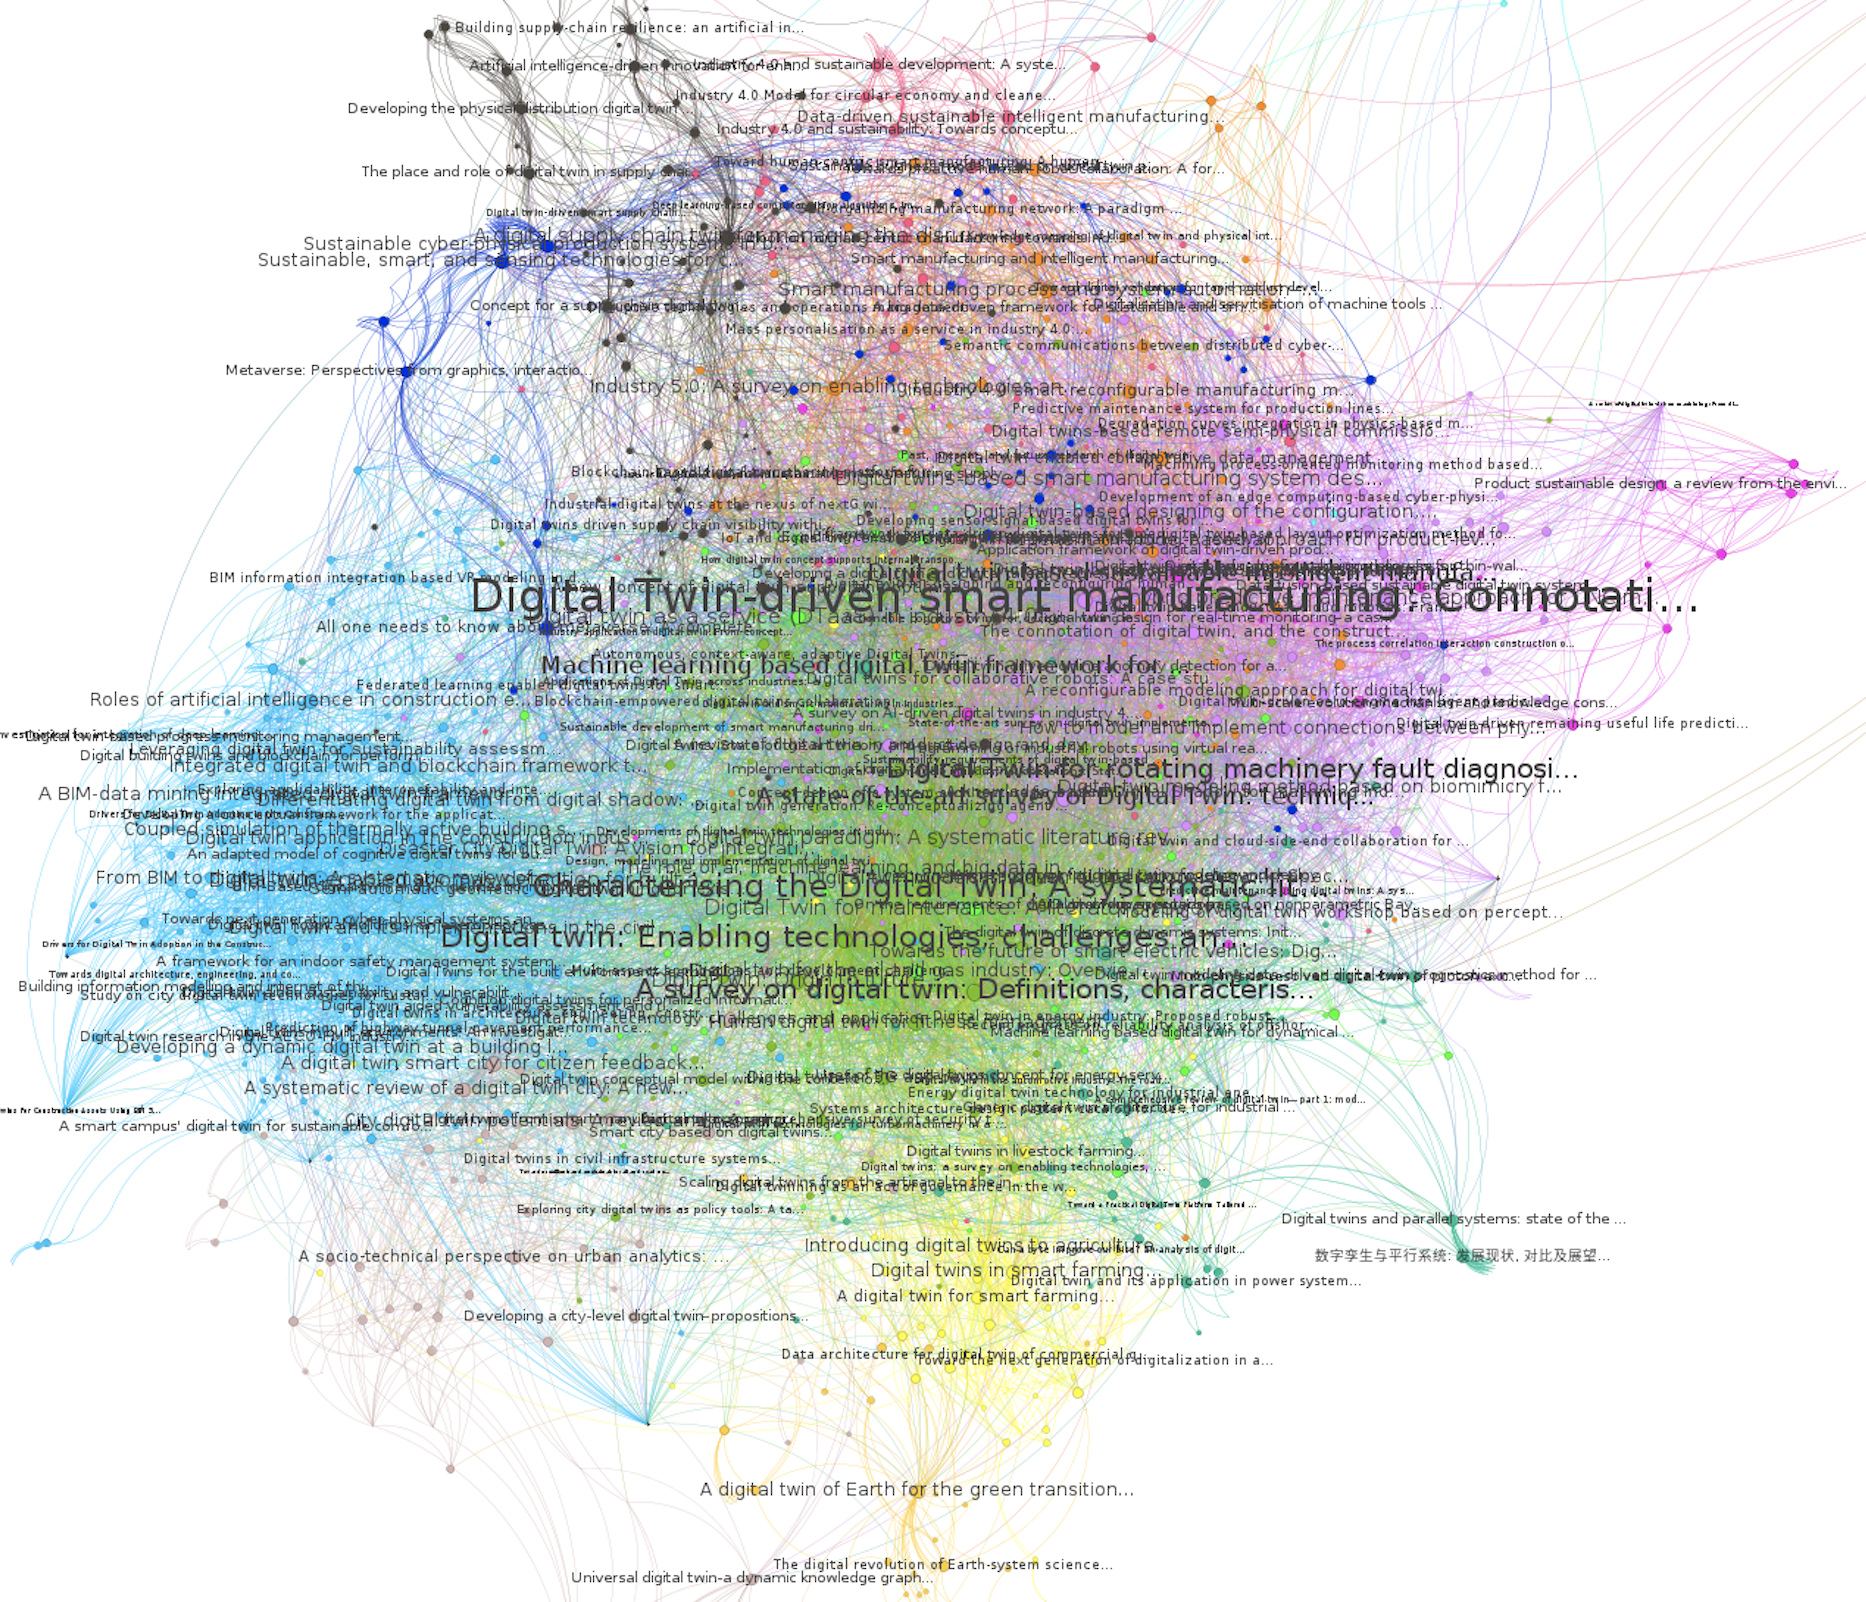
\includegraphics[width=1.1\linewidth]{figures/core_zoom}
	\end{column}
	\begin{column}{0.39\linewidth}
		\footnotesize
		\begin{itemize}
		    \item ``Smart manufacturing'' (21.9\%)
			\item Epistemology of DT (14.6\%)
			\item Civil engineering/BIM (11.4\%)
			\item Supply chain (6.8\%)
			\item Circular economy (5.6\%)
			\item Energy systems (5.1\%)
			\item Urban analytics/smart cities (5.0\%)
			\item ``Metaverse'' (4.5\%)
			\item ``Industry 4.0'' (4.2\%)
			\item ``Smart farming'' (4.0\%)
		\end{itemize}
	\end{column}
\end{columns}



}





\sframe{Digital twins: concepts and reality}{

\justify

% dig twins \cite{batty2018digital}

\textbf{Definition of a DT?} Coined in the 2000s from engineering \cite{batty2018digital}

\medskip

{\footnotesize ``\textit{A digital twin is a mirror image of a physical process [\ldots], usually matching exactly the operation of the physical process which takes place in real time.}''}

\medskip

$\rightarrow$ in practice not identical (example for cities: real-time GIS \cite{li2020real}); often not in real time or even dynamical.

\bigskip

The \textbf{link between the model (twin) and the system} is complex: which level of detail, which modelling choices, how to handle the resulting hybrid cyber-physical system? \cite{batty2019map}

``{\footnotesize \textit{A map is not the territory, or is it?}}''
% (inspire houllebeq et Levy) (meaning of representation)

\bigskip

% link with complexity \cite{arcaute2021future}

DT approaches too close to systems engineering, and often miss \textbf{social science/complexity} issues \cite{arcaute2021future}

$\rightarrow$ models at all time scales decision-making in the anthropocene.


}



\sframe{From digital twins to multiple simulation models}{


\justify

\textit{How to link digital twins and decision-making for sustainable development?}

\bigskip
\bigskip

$\rightarrow$ smart cities are on the long run: urban analytics for policy \\
\cite{kandt2021smart}

\bigskip

$\rightarrow$ unpredictability, multi-dimensionality, multi-scalarity of territorial systems: need for multiple models \cite{batty2021multiple}, multiple perspectives\\
 \cite{pumain2020conclusion}

\bigskip

$\rightarrow$ simulation models of territories for sustainable policies\\
\cite{raimbault2020empowering}


}









\sframe{Model integration: land-use transport interactions}{


\includegraphics[width=0.39\linewidth]{figures/accessp_withbridge_prd_EN.png}
\includegraphics[width=0.6\textwidth]{figures/macrocoevol_en.png}

\medskip


\textit{A modeling approach to the issue of structuring effects of transport infrastructures: co-evolution of networks and territories as a strong model integration}

\bigskip

\tiny
%\textcolor{grey}
Raimbault, J. (2019). Evolving accessibility landscapes: mutations of transportation networks in China. In Aveline-Dubach, N., ed. \textit{Pathways of sustainable urban development across China - the cases of Hangzhou, Datong and Zhuhai}, pp 89-108. Imago. ISBN:978-88-94384-71-0

\nocite{raimbault:halshs-02265423}

\smallskip

Raimbault, J. (2020). Indirect evidence of network effects in a system of cities. Environment and Planning B: Urban Analytics and City Science, 47(1), 138-155.

\nocite{raimbault2020indirect}

\smallskip

Raimbault, J. (2021). Modeling the co-evolution of cities and networks. In Handbook of Cities and Networks. Edward Elgar Publishing.

\nocite{raimbault2021modeling}


}


\sframe{Implementing horizontal model integration}{

\justify

\textit{Constructing a multimodal four step transport models by linking open components and data with scientific workflow engines}

\bigskip

\textbf{Integrated models:}

\begin{itemize}
	\item MATSim model (MATSim Community) for transport \cite{w2016multi}
	\item SPENSER model (University of Leeds) for synthetic population \cite{spooner2021dynamic}
	\item QUANT model (CASA, University College London) for spatial interactions \cite{batty2021new}
	\item spatialdata library (OpenMOLE community) for data processing \cite{raimbault2020scala}
\end{itemize}

\smallskip

\tiny

Raimbault, J., \& Batty, M. (2021). Estimating public transport congestion in UK urban areas with open transport models. GISRUK 2021 Proceedings.

\nocite{raimbault2021estimating}

}


\sframe{Model coupling: urban design and UHI}{

\begin{columns}
	\begin{column}{0.6\linewidth}
		\begin{center}
			\includegraphics[width=\linewidth]{figures/buildings_6.png}	
		\end{center}
	\end{column}
	\begin{column}{0.39\linewidth}
		\justify
		\textbf{SURe project} (collaboration LASTIG, ISC-PIF, EPIDAPO)
		
		\bigskip
		
		$\rightarrow$ coupling the SimPLU3D urban generative model \cite{brasebin2017apports} with an Urban Heat Island model to find compromises between density and the UHI effect. 

	\end{column}
\end{columns}




}


















